%------------------------------------------------------------------------
%Gestionar Colaboradores
\hypertarget{cv:GestionarColaboradores}{\section{Gestionar Colaboradores}} \label{sec:GestionarColaboradores}

	Esta funcionalidad le permitirá consultar los colaboradores que se encuentran registrados en el sistema los cuales podrán participar dentro de los proyectos que se vayan creando dentro del TESSERACT.

		\subsection{Procedimiento}

			%Pasos de procedimiento
			\begin{enumerate}
	
			\item Seleccione la opción \textbf{Colaboradores} del menú \ref{fig:MN-AD}.
	
			\item Se mostrará la pantalla \ref{fig:GestionarColaboradores} ''Gestionar Colaboradores''.

			%Pantalla
			\begin{figure}[htbp!]
				\begin{center}
					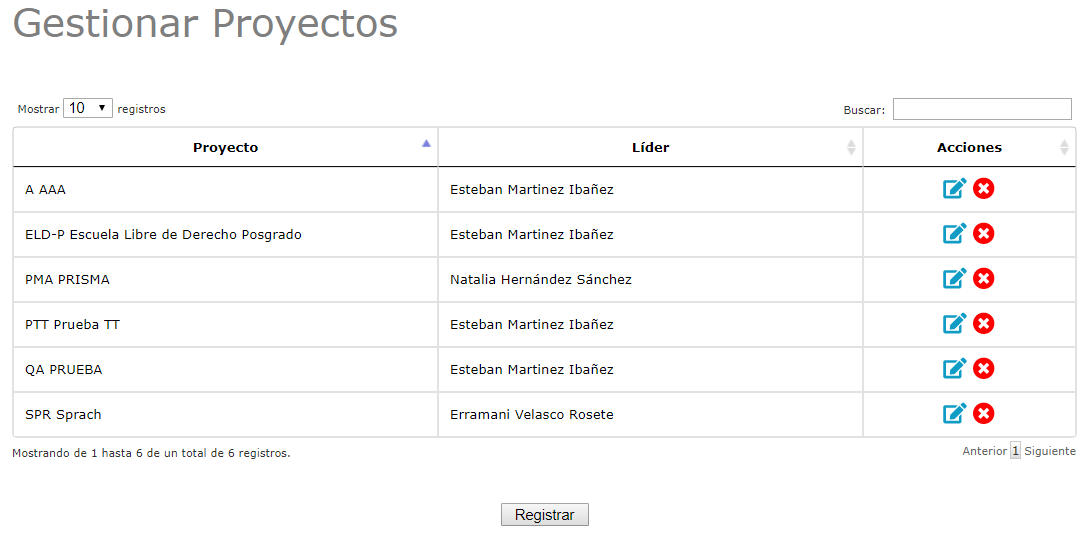
\includegraphics[scale=0.5]{images/inicioSesion/IU2GestionProyectos}
					\caption{Gestionar Colaboradores}
					\label{fig:GestionarColaboradores}
				\end{center}
			\end{figure}
		
			\item Seleccione la operación que desea realizar:
			
			Para (\hyperlink{cv:registrarColaborador}{Registrar}) dé clic en el botón \IURegistrar.
			
			Para (\hyperlink{cv:modificarColaborador}{Modificar}) dé clic en el icono \IUEditar{} de algún colaborador ya registrado.
			
			Para (\hyperlink{cv:VisualizarTrayDocente_SP}{Eliminar}) dé clic en el icono \IUBotonEliminar{} de algún colaborador ya registrado. 
			
			
			\end{enumerate}